\documentclass[10pt]{article}
\usepackage[letterpaper]{geometry}
\geometry{verbose,tmargin=1in,bmargin=1in,lmargin=1in,rmargin=1in}
\usepackage{setspace}
\usepackage{ragged2e}
\usepackage{color}
\usepackage{titlesec}
\usepackage{graphicx}
\usepackage{float}
\usepackage{mathtools}
\usepackage{amsmath}
\usepackage[font=small,labelfont=bf,labelsep=period]{caption}
\usepackage[english]{babel}
\usepackage{indentfirst}
\usepackage{array}
\usepackage{makecell}
\usepackage[usenames,dvipsnames]{xcolor}
\usepackage{multirow}
\usepackage{tabularx}
\usepackage{arydshln}
\usepackage{caption}
\usepackage{subcaption}
\usepackage{xfrac}
\usepackage{etoolbox}
\usepackage{cite}
\usepackage{url}
\usepackage{dcolumn}
\usepackage{hyperref}
\usepackage{courier}
\usepackage{url}
\usepackage{esvect}
\usepackage{commath}
\usepackage{verbatim} % for block comments
\usepackage{enumitem}
\usepackage{hyperref} % for clickable table of contents
\usepackage{braket}
\usepackage{titlesec}
\usepackage{booktabs}
\usepackage{gensymb}
\usepackage{longtable}
\usepackage{listings}
\usepackage{cancel}
\usepackage{tcolorbox}
\usepackage[mathscr]{euscript}
\lstset{
	basicstyle=\ttfamily\small,
    frame=single,
    language=fortran,
    breaklines=true,
    commentstyle=\color{magenta}\ttfamily,
    postbreak=\raisebox{0ex}[0ex][0ex]{\ensuremath{\color{red}\hookrightarrow\space}}
}

% for circled numbers
\usepackage{tikz}
\newcommand*\circled[1]{\tikz[baseline=(char.base)]{
            \node[shape=circle,draw,inner sep=2pt] (char) {#1};}}

\newcommand{\beq}{\begin{equation}}
\newcommand{\eeq}{\end{equation}}
\newcommand{\beqa}{\begin{equation}\begin{aligned}}
\newcommand{\eeqa}{\end{aligned}\end{equation}}

\titleclass{\subsubsubsection}{straight}[\subsection]

% define new command for triple sub sections
\newcounter{subsubsubsection}[subsubsection]
\renewcommand\thesubsubsubsection{\thesubsubsection.\arabic{subsubsubsection}}
\renewcommand\theparagraph{\thesubsubsubsection.\arabic{paragraph}} % optional; useful if paragraphs are to be numbered

\titleformat{\subsubsubsection}
  {\normalfont\normalsize\bfseries}{\thesubsubsubsection}{1em}{}
\titlespacing*{\subsubsubsection}
{0pt}{3.25ex plus 1ex minus .2ex}{1.5ex plus .2ex}

\makeatletter
\renewcommand\paragraph{\@startsection{paragraph}{5}{\z@}%
  {3.25ex \@plus1ex \@minus.2ex}%
  {-1em}%
  {\normalfont\normalsize\bfseries}}
\renewcommand\subparagraph{\@startsection{subparagraph}{6}{\parindent}%
  {3.25ex \@plus1ex \@minus .2ex}%
  {-1em}%
  {\normalfont\normalsize\bfseries}}
\def\toclevel@subsubsubsection{4}
\def\toclevel@paragraph{5}
\def\toclevel@paragraph{6}
\def\l@subsubsubsection{\@dottedtocline{4}{7em}{4em}}
\def\l@paragraph{\@dottedtocline{5}{10em}{5em}}
\def\l@subparagraph{\@dottedtocline{6}{14em}{6em}}
\makeatother

\newcommand{\volume}{\mathop{\ooalign{\hfil$V$\hfil\cr\kern0.08em--\hfil\cr}}\nolimits}

\setcounter{secnumdepth}{4}
\setcounter{tocdepth}{4}

\title{MPI Parallelization of a Finite Element Application}
\author{April Novak}


\begin{document}
\maketitle

\section{Introduction}

This final project for CS-267 involves the serial creation and parallelization of a finite element solver to the heat equation, which in its simplest form describes the diffusion of temperature with a heat source:

\beq
\label{eq:eq}
-k\frac{\partial^2 T}{\partial x^2}=\dot{q}
\eeq

where \(k\) is the thermal conductivity, \(T\) is the temperature, and \(\dot{q}\) is a volumetric heat source. This equation is kept very simple so that the goals of the project can focus entirely on parallelization algorithms, rather than more advanced numerical methods for solving convection-diffusion equations that would be encountered in a class such as MATH-228b (Numerical Solutions of Differential Equations). Due to the second derivative present in this equation, in 1-D, two boundary conditions are needed on both ends of the domain, and in 2-D, boundary conditions must be known on the entire perimeter. This presents the fundamental difficulty of parallelizing a numerical solution to this equation - if the domain is divided amongst different parallel processes or threads, then the equations cannot be solved unless guesses are made for the conditions on the boundaries that are created upon domain decomposition. Hence, any parallel solution will require an iterative procedure, where an initial guess for the interior boundary conditions are continually updated by comparing results obtained at processor-interfaces. Hence, this application is \textit{not} embarrassingly parallel, and if the number of iterations required to reach convergence is very large, then the parallel runtime can easily be longer than the serial runtime. Hence, clever parallel algorithms will be developed such that a net reduction in runtime and good strong and weak scaling can be obtained for this numerical solution.

From the point of view of parallelization algorithms, the numerical method chosen can have a large impact on the success of strong and weak scaling results. For this project, the finite element method is chosen as the ODE solver because my research focuses on finite element methods applied to the field of Computational Fluid Dynamics (CFD). This assignment solves the heat equation in 1-D, and time permitting, will also pursue 2-D solutions. The remainder of this section will discuss the numerical method applied to the heat equation in 1-D, and some familiarity with numerical methods is assumed so that the brunt of this report can focus on parallelization rather than numerical methods. A similar approach to homework 2 is pursued here, in that effort is first spent on obtaining fast serial code, followed by the introduction of parallel algorithms to obtain good strong and weak scaling.

The finite element method (FEM) is a weighted residual method, that for parabolic equations can be shown to be optimal in the energy norm (i.e. the FEM solution will outperform {\it all} other solutions when measured in this norm). By multiplying Eq. \eqref{eq:eq} by a test function \(\psi\) and integrating over all space, we obtain the weak form:

\beqa
-\int_{\Omega}k\frac{\partial^2 T}{\partial x^2}\psi(x)dx=&\int_{\Omega}\dot{q}\psi(x)dx\\
\int_{\Omega}\frac{\partial T}{\partial x}k\frac{\partial\psi(x)}{\partial x}dx-\int_{\Gamma}k\frac{\partial T}{\partial x}\psi(x)\cdot\hat{n}dx=&\int_{\Omega}\dot{q}\psi(x)dx\\
\eeqa

where \(\Omega\) indicates the entire domain and \(\Gamma\) the boundary of the domain. Integration by parts has been applied in the second form above to transfer some differentiation from the solution variable \(T\) to the test function \(\psi\). This allows {\it weaker} differentiability requirements for our numerical representation of \(T\), since now the integral only requires that \(T\) be continuous (rather than differentiable as well). Now, an assumption about the form of the solution is made. We assume that the numerical solution \(T_h\) (subscript \(h\) refers to an element of width \(h\)) is a sum of coefficients multiplied by expansion functions \(\phi\):

\beq
T_h=\sum_{j=1}^{N}c_j\phi_j(x)
\eeq

where there are \(N\) of these expansion functions defined over the entire domain. Hence, the numerical method reduces to the problem of determining the expansion coefficietns \(c_j\) for a user-selected set of \(\phi_j(x)\). For parabolic equations, the Galerkin FEM specifies that \(\psi\) should come from the same space as \(T_h\). Hence, inserting these expansions into the weak form gives:

\beqa
\int_{\Omega}\frac{\partial \sum_{j=1}^Nc_j\phi_j(x)}{\partial x}k\frac{\partial\sum_{i=1}^Nb_i\phi_i(x)}{\partial x}dx-\int_{\Gamma}k\frac{\partial \sum_{j=1}^Nc_j\phi_j(x)}{\partial x}\sum_{i=1}^N\phi_i(x)\cdot\hat{n}dx=&\int_{\Omega}\dot{q}\sum_{i=1}^Nb_i\phi_i(x)dx\\
\int_{\Omega}\frac{\partial \sum_{j=1}^Nc_j\phi_j(x)}{\partial x}k\frac{\partial\sum_{i=1}^N\phi_i(x)}{\partial x}dx-\int_{\Gamma}k\frac{\partial \sum_{j=1}^Nc_j\phi_j(x)}{\partial x}\sum_{i=1}^N\phi_i(x)\cdot\hat{n}dx=&\int_{\Omega}\dot{q}\sum_{i=1}^N\phi_i(x)dx\\
\eeqa

where the coefficients \(b_i\) can be cancelled from each term because they are arbitrary. While this equation holds for \(i=1, N\) and \(j=1, N\), it is true that it also holds for each individual selection of \(i\) and \(j\). This stronger requirements allows the summation terms to be removed, with the implication that we have changed one equation to \(N\) equations:

\beqa
c_j\int_{\Omega}\frac{\partial \phi_j(x)}{\partial x}k\frac{\partial\phi_i(x)}{\partial x}dx-c_j\int_{\Gamma}k\frac{\partial \phi_j(x)}{\partial x}\phi_i(x)\cdot\hat{n}dx=&\int_{\Omega}\dot{q}\phi_i(x)dx\\
\eeqa

The above can be written in more concise form using matrix notation. The stiffness matrix \textbf{K} is:

\beq
\label{eq:k}
K_{ij}=\int_{\Omega}\frac{\partial \phi_j(x)}{\partial x}k\frac{\partial\phi_i(x)}{\partial x}dx-\int_{\Gamma}k\frac{\partial \phi_j(x)}{\partial x}\phi_i(x)\cdot\hat{n}dx
\eeq

and the load vector \(\textbf{R}\) is:

\beq
R_{i}=\int_{\Omega}\dot{q}\phi_i(x)dx
\eeq

which gives a set of linear equations that is solved for \(c_j\):

\beq
K_{ij}c_j=R_i
\eeq

The stiffness matrix consists of the multiplication of the derivatives of \(\phi_i(x)\) with \(\phi_j(x)\). If these shape functions are defined over the {\tt entire} domain, then the stiffness matrix will be a dense matrix. On the other hand, if we choose these shape functions to be nonzero only over a single small region of the domain, then the product of cross terms will be zero for most of the matrix, since the effect of a single shape function will be very localized. This will produce sparse matrices, which will be much easier to work with and will also permit easier extension as a numerical method over a discretized domain. Hence, the expansion for the solution and test function for a {\it single} element (``element'' is used in this sense as a small region of the domain, i.e. a meshing software would divide up a continuous domain into discrete elements) becomes:

\beq
T_h^e=\sum_{j=1}^{n_{en}}c_j^e\phi_j^e(x)
\eeq

where the \(e\) superscript indicates the element and \(n_{en}\) are the number of element nodes. A nodal basis is selected for the shape functions. This means that, over a single element, the shape functions are unity at their corresponding node, and zero at the other nodes. The matrix equation \(K_{ij}c_j=R_i\) can be written for written for each individual element, with a post-processing step that takes the system of equations for each element and connects them all together to enforce solution continuity at element interfaces. 

\beq
K_{ij}^ec_j^e=R_i^e
\eeq

where

\beq
K_{ij}^e=\int_{\Omega^e}\frac{\partial \phi_j(x)}{\partial x}k\frac{\partial\phi_i(x)}{\partial x}dx-\int_{\Gamma^e}k\frac{\partial \phi_j(x)}{\partial x}\phi_i(x)\cdot\hat{n}dx
\eeq

\beq
R_{i}^e=\int_{\Omega^e}\dot{q}\phi_i(x)dx
\eeq

such that the domain of integration is only over a single element. However, the system of equations for each element, \(K_{ij}^ec_j^e=R_i^e\), is singular, and cannot be solved independently of the other elements, since we require solution continuity at inter-element nodes. So, the elemental system of equations must be assembled into the global system of equations using a location matrix that dictates how the global nodes in the entire mesh relate to the local node numbering in each finite element. Figure \ref{fig:FEmesh} shows a simple FE mesh, where the numbers illustrate the global node numbering. A mapping is required from the elemental perspective to this global mesh. The location matrix contains this information - each column of the location matrix gives the global node numbers that correspond to the local node numbers. The local nodes must always be numbered in a consistent manner (i.e. always clockwise or always counterclockwise) so that the Jacobian of the local to global transformation is positive. The first five columns of the location matrix for this mesh, for illustration, would be:

\beq
\label{eq:LM}
LM=\begin{bmatrix}
1 & 2 & 3 & 4 & 5 & \cdots\\
2 & 3 & 4 & 5 & 6 & \cdots\\
11 & 12 & 13 & 14 & 15 & \cdots\\
10 & 11 & 12 & 13 & 14 & \cdots\\
\end{bmatrix}
\eeq

where the nodes have been numbered counterclockwise.

\begin{figure}[H]
\centering
\includegraphics[width=0.8\textwidth]{../figures/FEmesh.pdf}
\caption{Global node numbering in a simple FE mesh. Source:\newline {\tt http://opensees.berkeley.edu/wiki/index.php/}\newline{\tt Simply\_supported\_beam\_modeled\_with\_two\_dimensional\_solid\_elements}}
\label{fig:FEmesh}
\end{figure}

For structured meshed, this location matrix is fairly easy to determine, but for unstructured meshes where there is not necessarily a pattern to the node connectivity, would be provided by a meshing software such as Cubit. Once this location matrix is known, the elemental systems of equations \(K_{ij}^ec_j^e=R_i^e\) can be assembled into the global system of equations \(K_{ij}c_j=R_i\). The fundamental reason why it is preferred to assemble the equations for each element individually, and {\tt then} assemble these into a global system, is that we have chosen shape functions that are only nonzero over an element and its immediate neighbors. This algorithm is inherently local until we get to the step requiring continuity, and it is hence natural to avoid unnecessary computations of zero integrals by only computing the integrals over each element, and then assembling these systems together at the end right before the numerical solve. For better illustration, several entries of \textbf{K} are assembled as follows for the location matrix given in Eq. \eqref{eq:LM}.

\beqa
K(1, 1) =& k(1, 1)^{e=1}\\
K(1, 2) =& k(1, 2)^{e=1}\\
K(2, 2) =& k(2, 2)^{e=1}+k(1, 1)^{e=2}\\
K(2, 11) =& k(2, 3)^{e=1}\\
K(12, 12) =& k(3, 3)^{e=2}+k(4, 4)^{e=3}\\
\eeqa

where a new notation of lowercase \(k\) representing \(K^e\) is used. Once the global matrix has been assembled, any Dirichlet boundary conditions must be applied (Neumann boundary conditions have naturally been applied by the form of the perimeter integral in Eq. \eqref{eq:k}. Dirichlet boundary conditions are strictly imposed by removing the Dirichlet nodes from the global matrix system. For a 1-D domain consisting of four linear elements (two nodes per element), the global matrix system \(\textbf{K}c=\textbf{R}\) before imposition of Dirichlet boundary conditions is:

\beq
\textbf{K}=
\begin{bmatrix}
k(1, 1)^{e=1} & k(1, 2)^{e=1} & 0 & 0 & 0\\
k(2, 1)^{e=1} & k(2, 2)^{e=1}+k(1, 1)^{e=2} & k(1, 2)^{e=2} & 0 & 0\\
0 & k(2, 1)^{e=2} & k(2, 2)^{e=2}+k(1, 1)^{e=3} & k(1, 2)^{e=3} & 0\\
0 & 0 & k(2, 1)^{e=3} & k(2, 2)^{e=3}+k(1, 1)^{e=4} & k(1, 2)^{e=4}\\
0 & 0 & 0 & k(2, 1)^{e=4} & k(2, 2)^{e=4}\\
\end{bmatrix}
\eeq

\beq
\textbf{R}=\begin{bmatrix}
R_1^{e=1} \\ R_2^{e=1}+R_1^{e=2}\\R_2^{e=2}+R_1^{e=3}\\R_2^{e=3}+R_1^{e=4}\\R_2^{e=4}\\
\end{bmatrix}
\eeq

To apply Dirichlet boundary conditions at nodes \(1\) and \(5\), the off-diagonal terms in the stiffness matrix are set to zero and the corresponding terms in the global load vector are set to the Dirichlet values. For instance, to impose Dirichlet conditions of \(T(node 1)=3.5\) and \(T(node 5) = 10.5\), the global matrix system becomes:

\beq
\textbf{K}=
\begin{bmatrix}
1 & 0 & 0 & 0 & 0\\
k(2, 1)^{e=1} & k(2, 2)^{e=1}+k(1, 1)^{e=2} & k(1, 2)^{e=2} & 0 & 0\\
0 & k(2, 1)^{e=2} & k(2, 2)^{e=2}+k(1, 1)^{e=3} & k(1, 2)^{e=3} & 0\\
0 & 0 & k(2, 1)^{e=3} & k(2, 2)^{e=3}+k(1, 1)^{e=4} & k(1, 2)^{e=4}\\
0 & 0 & 0 & 0 & 1\\
\end{bmatrix}
\eeq

\beq
\textbf{R}=\begin{bmatrix}
3.5\\ R_2^{e=1}+R_1^{e=2}\\R_2^{e=2}+R_1^{e=3}\\R_2^{e=3}+R_1^{e=4}\\10.5\\
\end{bmatrix}
\eeq

Once these boundary conditions have been incorporated into the matrix system, the matrix system can be solved by your favorite linear algebra routine. For this assignment, the Conjugate Gradient (CG) method is selected to solve this symmetric system because this will provide more flexibility for exploring parallelization algorithms than simply using some routine from BLAS or LAPACK. To solve a matrix system \(\textbf{K}a=R\) by the CG method requires rewriting the governing equation as the minimization of a potential \(\Pi\) (recall from elementary physics classes that you can equivalently state that a system is balance by the sum of the forces equalling zero, {\it or} the total energy of the system being minimized). 

\beq
\label{eq:IterativeMethodsPotential}
\Pi=\frac{1}{2}a^T\textbf{K}a-a^TR
\eeq

The exact solution is obtained by taking the gradient of this potential with respect to each of the expansion coefficients in the vector \(a\), and setting that gradient equal to zero:

\beq
\frac{\partial\Pi}{\partial a}=\textbf{K}a-R=0
\eeq

This is not different than simply solving the original matrix system \(\textbf{K}a-R=0\). So, the minimizer to the potential \(\Pi\) is also a solution to the matrix system. Krylov methods are a class of methods that successively update an initial iterate guess in ways that minimize \(\Pi\) with each iteration. This minimization takes place over a vector space, called a Krylov space. These methods require computation of the residual:

\beq
r^i=R-\textbf{K}a^i
\eeq

where \(i\) is the iteration index. The CG method, while used as an iterative method, is technically a direct method if applied \(N\) times with perfect precision. Each update to the solution iterates is performed according to:

\beq
\label{eq:CGUpdate}
a^{i+1}=a^i+\lambda^iz^i
\eeq

where the update scales by \(z^i\):

\beq
\label{eq:ZUpdateCG}
z^i=r^i+\theta^iz^{i-1}
\eeq

where \(\theta^i\) is a parameter chosen such that \(z^i\) is \(\textbf{K}\)-conjugate to \(z^{i-1}\), or:

\beq
\label{eq:kconjugate}
z^{T,i}\textbf{K}z^{i-1}=0
\eeq

In other words, the search direction is a combination of a move in the reverse direction of the gradient (method of steepest descent) plus a motion perpendicular to that direction. This helps to avoid duplicate searching in the same general area. For the very first iteration, it is common to select \(z^1=r^1\). Simply plugging in Eq. \eqref{eq:ZUpdateCG} to Eq. \eqref{eq:kconjugate} gives:

\beq
\theta^i=-\frac{r^{T,i}\textbf{K}z^{i-1}}{z^{T,i-1}\textbf{K}z^{i-1}}
\eeq

Plugging in Eq. \eqref{eq:CGUpdate} into Eq. \eqref{eq:IterativeMethodsPotential} and then taking the partial derivative with respect to \(\lambda^i\), the optimal \(\lambda^i\) is:

\beq
\label{eq:UpdateCG}
\lambda^i=\frac{z^{T,i}r^i}{z^{T,i}\textbf{K}z^i}
\eeq

So, given an initial guess for the solution \(a\), CG iterations are performed until there is acceptably small difference between two successive iterates \(a^i\) and \(a^{i+1}\). This numerical method is selected due to its relative simplicity. This concludes the theoretical discussion of the FEM applied to this simple 1-D heat equation. The next section discusses steps taken to obtain a fast serial implementation of this algorithm, and will go into more detail regarding exactly how this method can be implemented in code.

\section{Serial Implementation}

This section discusses the serial code that is used as a launching point for parallel algorithms. As a nuclear engineering graduate student interested in computational methods, you will quickly learn that the consequences of errors in neutron transport codes used to design nuclear reactors can potentially be very high. For instance, the criticality of a nuclear reactor is expressed as an eigenvalue of the neutron transport equation - when this eigenvalue equals 1.0, the system is critical, and a safe, self-sustaining chain reaction can be obtained. However, if this eigenvalue is 1.0065, the system is supercritical, and without safety systems, a runaway chain reaction can result and be very dangerous. These tight design margins require very accurate modeling codes. Hence, in the nuclear power field, there is very slow acceptance of new modeling codes, since each new code must undergo rigorous verification and validation. Due to this feature, {\it many} nuclear simulation codes are written in Fortran, though there is an ongoing effort to convert legacy codes to more modern languages. So, I used this project as an opportunity to learn how to program in Fortran 2003. 

The serial code allows the user to input the domain length, number of finite elements, order of the interpolation, and domain Dirichlet boundary conditions from the command line. Then, several problem parameters such as the number of total nodes are computed. For the purpose of computing integrals, Gaussian quadrature is used. Because these quadrature points and weights are held fixed throughout the entire simulation, they only need to be initialized one time. All elementary integrals (over \(\Omega^e\)) are computed in a master element defined over \(-1\leq\xi\leq1\), rather than \(a\leq x\leq b\) in the physical domain. Hence, the elementary integrals are computed in this master element using the Jacobian of the transformation \(\mathscr{J}\):

\beq
\mathscr{J}=\frac{dx}{d\xi}=\frac{h}{2}
\eeq

where \(h\) is the element length in the physical domain and 2 the length in the master domain. Likewise, instead of defining shape functions individually for each finite element, they can be defined {\it once} in the master domain. Then, the elementary stiffness matrix and load vector become:

\beq
K_{ij}^e=\int_{-1}^{1}\frac{\partial \phi_j(\xi)}{\partial \xi}k\frac{\partial\phi_i(\xi)}{\partial \xi}\frac{1}{\mathscr{J}}d\xi-\int_{\Gamma^e}k\frac{\partial \phi_j(\xi)}{\partial \xi}\phi_i(\xi)\cdot\hat{n}d\xi
\eeq

\beq
R_{i}^e=\int_{-1}^{1}\dot{q}\phi_i(\xi)\mathscr{J}d\xi
\eeq

For linear elements, these nodal shape functions are:

\beqa
\phi_1(\xi)=\frac{1-\xi}{2}\\
\phi_2(\xi)=\frac{1+\xi}{2}\\
\eeqa

Higher-order shape functions can also easily be defined. These integrals are computed using Gaussian quadrature:

\beq
K_{ij}^e\approx\sum_{p=1}^{P}w_p\frac{\partial \phi_j(\xi_p)}{\partial \xi}k\frac{\partial\phi_i(\xi_p)}{\partial \xi}\frac{1}{\mathscr{J}}
\eeq

\beq
R_{i}^e\approx\sum_{p=1}^{P}w_p\dot{q}\phi_i(\xi_p)\mathscr{J}
\eeq

Because these quadrature points don't change throughout the simulation, the evaluation of the shape functions and their first derivatives at these quadrature points only needs to be determined once. In previous classes I have taken on the FEM, I had never made this connection, and had wasted flops re-computing these for every finite element. These values are stored in arrays {\tt phi} and {\tt dphi}, where each column pertains to an element, and each row to a quadrature point. These arrays are organized as such because the loops that assemble the global stiffness matrix and load vector loop over elements as the outermost loop. Because Fortran stores arrays in a column-major format, this should allow accesses to elements of the {\tt phi} and {\tt dphi} arrays faster.

\begin{lstlisting}
subroutine phi_val(order, qp)
  implicit none
  integer,  intent(in)  :: order
  real(rk), intent(in)  :: qp(:)

  ! only linear and quadratic elements are supported
  select case(order)
    case(1)
      phi(1, :)  = (1.0 - qp(:)) / 2.0
      phi(2, :)  = (1.0 + qp(:)) / 2.0
      dphi(1, :) = -1.0 / 2.0
      dphi(2, :) =  1.0 / 2.0
    case(2)
      phi(1, :)  = qp(:) * (qp(:) - 1.0) / 2.0
      phi(2, :)  = (1.0 - qp(:)) * (1.0 + qp(:))
      phi(3, :)  = qp(:) * (qp(:) + 1.0) / 2.0
      dphi(1, :) = (2.0 * qp(:) - 1.0) / 2.0
      dphi(2, :) = 1.0 - qp(:) * qp(:)
      dphi(3, :) = (2.0 * qp(:) + 1.0) / 2.0
    case default
      write(*,*) "phi and dphi not initialized due to polynomial order not being supported."
  end select
end subroutine phi_val
\end{lstlisting}

\(k\) and \(\dot{q}\) are assumed constant, which is a good approximation for nuclear applications where the thermal conductivity of the fuel changes slowly with fuel depletion and the heat source is kept constant through operator changes such as moving control rods in the reactor core. Then, the elemental stiffness matrix and load vector are computed, which will be the same for every element since \(k\) and \(\dot{q}\) are constant, and equal-sized elements are used. This is performed by looping over the quadrature points, and then over the {\tt i} and {\tt j} indices. 

\begin{lstlisting}
kel = 0.0
rel = 0.0
do q = 1, n_qp ! sum over quadrature points
  do i = 1, n_en
    rel(i) = rel(i) + wt(q) * source * phi(i, q) * h *h / 2.0
    do j = 1, n_en
      kel(i, j) = kel(i, j) + wt(q) * dphi(i, q) * k * dphi(j, q) * 2.0
    end do
  end do
end do
\end{lstlisting}

Because structured meshes are used, the location matrix is next defined, which can be defined in an analytical way due to the simplicity of the mesh.

\begin{lstlisting}
subroutine locationmatrix()
  implicit none
  integer :: i, j

  ! analytical form for 1-D elements
  do j = 1, n_el
    do i = 1, n_en
      LM(i, j) = (j - 1) * (n_en - 1) + i
    end do
  end do
end subroutine locationmatrix
\end{lstlisting}

The global load vector is formed by looping over the elements in the outermost loop such that the entries in the location matrix are accessed in a column major format. Dirichlet boundary conditions are imposed by manipulating the first and last entries (since the nodes are numbered in an ascending way such that node 1 and node {\tt n\_nodes} are on the boundaries).

\begin{lstlisting}
rglob = 0.0
do q = 1, n_el ! loop over the elements
  do i = 1, n_en
    rglob(LM(i, q)) = rglob(LM(i, q)) + rel(i)
  end do
end do

! apply boundary conditions
rglob(1) = leftBC ! left BC value
rglob(n_nodes) = rightBC ! right BC value
\end{lstlisting}

At this point, no global stiffness matrix has been formed - only the global load vector. Originally, I wrote code that assembled the global stiffness matrix, but because this matrix is sparse, this wastes a huge amount of memory in the storage of zeros. Instead, the global stiffness matrix does not need to be formed at all, since all that is required of the CG method is the {\it product} of the global stiffness matrix with a vector. The location matrix tells us which entries of the global stiffness matrix will be nonzero, so I developed a new function {\tt sparse\_mult} that takes as input an elementary stiffness matrix, a location matrix, and the vector with which to multiply the sparse matrix. By looping over the elements, an entry in the {\tt (i, j)} location of the {\it elementary} stiffness matrix will be placed in the {\tt (LM(i, element), LM(j, element))} location. Hence, for each entry of the elementary stiffness matrix, the product {\tt kel(i, j) * vector(LM(j, element))} will be placed into the {\tt LM(i, element)} entry of the resulting vector. Boundary conditions are natively applied within this function by recognizing that, in rows corresponding to the boundary conditions, diagonal terms must be set to zero and off-diagonal terms to 1.0. A kronecker-delta function performs this, which requires that for each occurrence of the innermost loop, an {\tt if}-statement be evaluated to determine if the current row of the global stiffness matrix matches one of the Dirichlet boundaries. Hence, this function completely eliminates the need to store the entire global stiffness matrix, which for linear elements represents a memory reduction of a factor of \(N_{el}\), where \(N_{el}\) is the number of elements. 

\begin{lstlisting}
function sparse_mult(matrix, LM, vector)
  implicit none
  real(rk) :: matrix(:, :) ! elementary matrix (assumed-shape array)
  real(rk) :: vector(:)    ! full vector (assumed-shape array)
  integer  :: LM(:, :)     ! location matrix

  real(rk) :: sparse_mult(size(vector))

  integer :: i, j, q
  
  sparse_mult = 0.0
  do q = 1, n_el ! loop over the elements
    do i = 1, n_en ! loop over all entries in kel
      do j = 1, n_en
        if (any(BCs == LM(i, q))) then
          ! apply boundary conditions
          ! diagonal terms set to 1.0, off-diagonal set to 0.0
          sparse_mult(LM(i, q)) = sparse_mult(LM(i, q)) + & 
            kronecker(LM(i, q), LM(j, q)) * 1.0 * vector(LM(j, q))
        else
          sparse_mult(LM(i, q)) = sparse_mult(LM(i, q)) + &
            matrix(i, j) * vector(LM(j, q))
        end if
      end do
    end do
  end do
end function sparse_mult
\end{lstlisting}

This function is used with the CG solver to perform repeated multiplications of the global stiffness matrix (never formed) with a vector. To make vectorization easier, I also created a function that computes the dot product of two vectors. 

\begin{lstlisting}
subroutine conjugategradient()
  ! perform very first iteration
  aprev = 1.0
  res = rglob - sparse_mult(kel, LM, aprev)
  zprev = res
  lambda = dotprod(zprev, res) / dotprod(zprev, sparse_mult(kel, LM, zprev))
  a = aprev + lambda * zprev
  convergence = 0.0

  ! compute error of first iteration to check if we nailed it first-try
  do i = 1, n_nodes
    convergence = convergence + abs(a(i) - aprev(i))
  end do

  ! loop until the error is lower than a specified tolerance
  do while (convergence > tol)
    ! update CG solution iterate
    aprev = a
    res = rglob - sparse_mult(kel, LM, aprev)
    theta = - dotprod(res, sparse_mult(kel, LM, zprev)) / &
      dotprod(zprev, sparse_mult(kel, LM, zprev))
    z = res + theta * zprev
    lambda = dotprod(z, res) / dotprod(z, sparse_mult(kel, LM, z))
    a = aprev + lambda * z
    zprev  = z

    convergence = 0.0
    ! recompute the error
    do i = 1, n_nodes
      convergence = convergence + abs(a(i) - aprev(i))
    end do

  end do
end subroutine conjugategradient
\end{lstlisting}

\begin{lstlisting}
real function dotprod(vec1, vec2)
  implicit none
  real(rk) :: vec1(:)
  real(rk) :: vec2(:)

  integer  :: i

  dotprod = 0.0
  do i = 1, size(vec1)
    dotprod = dotprod + vec1(i) * vec2(i)
  end do
end function dotprod
\end{lstlisting}

This concludes the basic description of the serial algorithm. To summarize, the main Fortran code, after allocations of memory for all of the arrays, looks like:

\begin{lstlisting}
! parse command line arguments
call commandline(length, n_el, order, leftBC, rightBC)

! initialize problem variables
call initialize(h, x, n_en, n_el, order, n_nodes)  

! initialize quadrature rule    
call quadrature(order, n_qp, qp, wt)      

! allocate memory for all of the necessary arrays             

! determine phi and d(phi)/dx in the master domain at the quadrature points
call phi_val(order, qp)

! form the location matrix
call locationmatrix()

! determine the boundary condition nodes
BCs = (/1, n_nodes/)

! form the elemental stiffness matrix and load vector
kel = 0.0
rel = 0.0
do q = 1, n_qp
  do i = 1, n_en
    rel(i) = rel(i) + wt(q) * source * phi(i, q) * h *h / 2.0
    do j = 1, n_en
      kel(i, j) = kel(i, j) + wt(q) * dphi(i, q) * k * dphi(j, q) * 2.0
    end do
  end do
end do

! form the global load vector
rglob = 0.0
do q = 1, n_el
  do i = 1, n_en
    rglob(LM(i, q)) = rglob(LM(i, q)) + rel(i)
  end do
end do

! apply boundary conditions
rglob(1) = leftBC
rglob(n_nodes) = rightBC

! perform CG solution
call conjugategradient()

deallocate(qp, wt, x, kel, rel, phi, dphi, rglob, a, aprev, z, zprev, res, LM)
\end{lstlisting}

The remainder of this section will discuss changes made to this serial algorithm just described in order to obtain better serial performance. With no compiler flags, the runtime of this serial code on 2.5 GHz Intel Core i5 is shown below for 1000 to 10000 finite elements. By measuring the runtime of the {\tt conjugategradient} subroutine, it can be seen that the total runtime is almost entirely due to the conjugate gradient solution. Hence, most effort will be spent optimizing this function. The number of CG iterations increases with the number of elements - without preconditioning, this cannot be changed and is a feature of the numerical method. However, what {\it can} be improved through code adjustments is the runtime per CG iteration, shown in Fig. \ref{fig:runtime_per_CG} below. As can be seen, the runtime for each CG iteration is not constant, and this is due to the fact that the larger the number of elements, the larger the matrix multiplications and vector dot products inherent to the iterative solver. A very simple change that can be done is to use a better starting guess for the iterative solution. By changing the initial guess from unity to a straight line between the left and right Dirichlet boundary conditions, the runtime per CG iteration drops by about a factor of 10 due to the factor of 10 lower iterations required due to being closer to the true numerical solution.

% better-initial-guess.txt : sets a better guess for a
\begin{figure}[H]
\centering
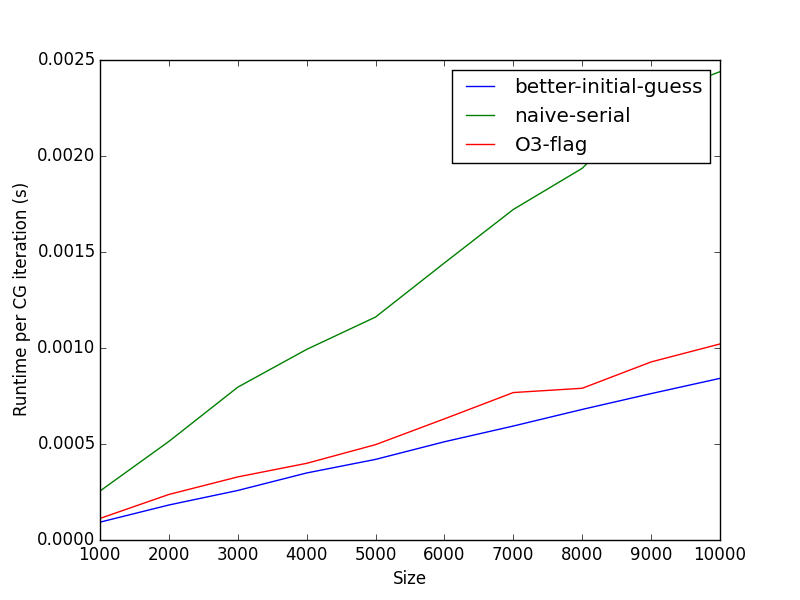
\includegraphics[width=0.6\linewidth]{../figures/O3-flag-runtime-per-CG.png}
\caption{Runtime per CG iteration as a function of the number of elements with the naive serial code (no compiler flags) and the same code compiled with the {\tt -O3} option. The same number of iterations are performed for each number of discrete elements.}
\end{figure}

A challenge associated with an iterative solution scheme is that it is not easily parallelizable - each iteration of the loop depends on previous solution iterates, and while the matrix multiplication and dot products can be easily parallelized, some quantities, such as \(\theta\) and \(\lambda\), require the aggregate matrix-vector products and vector-vector products, and hence the entire iterative solution cannot be performed completely independently for sections of the numerical solution.

\subsection{Reducing FLOPs}
The first, and perhaps most obvious, way to improve performance is to reduce unnecessary computation. This can be done in the {\tt conjugategradient} function by not performing {\tt sparse_mult} 

\subsection{Vectorization}

Single Instruction, Multiple Data (SIMD) is the process by which a single instruction is used to perform an operation on multiple pieces of data at the same time. When instructed with the appropriate vectorization flags, the compiler will try to find SIMD parallelism and use them as much as possible. Because a register only consists of a limited number of bytes, the degree of parallelism achievable is dependent on the data type of the variable that is being operated on. If a register contains 16 bytes, then because doubles are 8 bytes, while floats are 4 bytes, you can only achieve 2x parallelism with doubles, but 4x parallelism with floats. Using the GNU compiler, automatic vectorization can be attempted using the {\tt -O3} flag. Using this flag, as opposed to zero compiler flags, yields a dramatic performance improvement. Fig. \ref{fig:O3-flag} shows the runtime as a function of the number of elements with the naive serial code (no compiler flags) and the same code compiled with the {\tt -O3} option.

% naive-serial.txt: original serial code version, with no vectorization or other optimizations made in the CG solver
% O3-dotprod.txt: original code compiled with -O3

\begin{figure}[H]
\centering
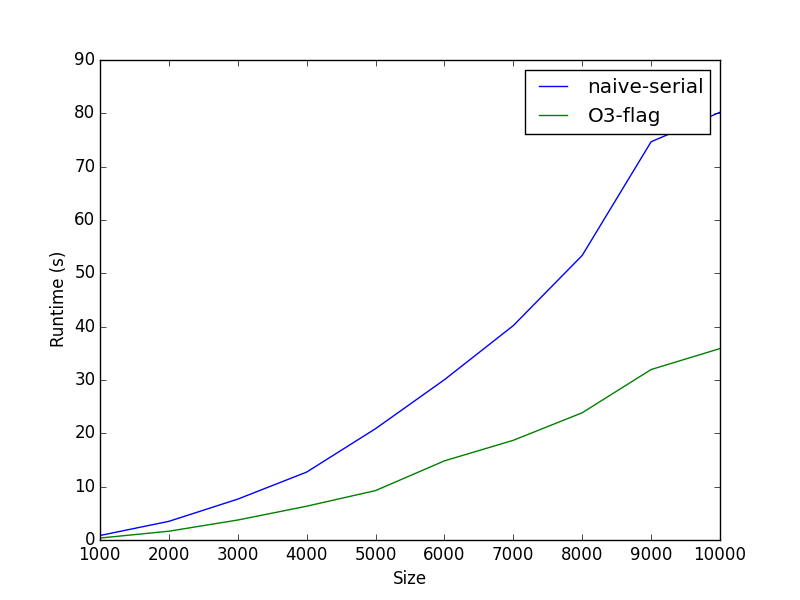
\includegraphics[width=0.6\linewidth]{../figures/O3-flag.png}
\caption{Runtime as a function of the number of elements with the naive serial code (no compiler flags) and the same code compiled with the {\tt -O3} option.}
\end{figure}

\section{Parallel Implementation}
This section discusses parallelization of the serial code developed in the previous section. In general, there are two very different parallelization strategies here - the first involves domain decomposition amongst parallel threads, where each parallel thread then runs a complete FEM solution, with iteration between threads until all threads agree on the values of the solution at the boundaries between the spatial domain allocated to each process. Alternatively, a single FEM problem can be run (with no need to iterate boundary conditions because the domain is not decomposed), and the work for the single FEM solve distributed amongst parallel instances.
\end{document}
